\documentclass[12pt]{article}
\usepackage{amsmath, amssymb}
\usepackage{graphicx}
\usepackage{tikz}
\usepackage[margin=1in]{geometry}
\usepackage{float} % For the H specifier

\title{Ejercicios de grafos}
\author{David Rivera Morales}
\date{\today}

\begin{document}

\maketitle

\section*{Problema 4}
Considera \( G \) una gráfica de orden \( n = 8 \) y tamaño \( m = 15 \) en la cual cada vértice es de grado 3 o 5. ¿Cuántos vértices de grado cinco tiene \( G \)?
\begin{enumerate}
    \item Supongamos que la gráfica \( G \) tiene \( x \) vértices de grado 5 y \( y \) vértices de grado 3.
    \item Dado que la gráfica tiene un total de \( n = 8 \) vértices, podemos establecer:
    \[ x + y = 8 \]
    (es decir, la suma de vértices de grado 5 y vértices de grado 3 es 8).
    \item Cada vértice de grado 5 contribuye con 5 aristas y cada vértice de grado 3 contribuye con 3 aristas. Pero, cada arista se cuenta dos veces (una vez por cada vértice que incide en ella). Por lo tanto, el total de aristas \( m \) es:
    \[ \frac{5x + 3y}{2} = 15 \]
    (es decir, la suma ponderada de los vértices de grado 5 y 3, dividido por 2, es igual al total de aristas).
    \item Ahora, tenemos un sistema de ecuaciones con dos incógnitas:
    \begin{align*}
    x + y &= 8 \quad (i) \\
    \frac{5x + 3y}{2} &= 15 \quad (ii)
    \end{align*}
    Resolviendo este sistema, encontramos que \( x = 3 \). Es decir, la gráfica \( G \) tiene 3 vértices de grado 5.
\end{enumerate}


\section*{Problema 5}
Dada la siguiente gráfica \( G' \):

\begin{enumerate}
    \item Encuentra una subgráfica generadora tal que todo vértice tenga grado 4.
          \begin{figure}[h]
              \centering
              \includegraphics[width=0.7\textwidth]{assets/g-prime.png}
              \caption{Gráfica \( G' \)}
              \label{fig:g-prime}
          \end{figure}

    \item Dibuja a la subgráfica inducida por \( A = \{u1, u2, u10, u4, u7, u8\} \).
          \begin{figure}[H]
              \centering
              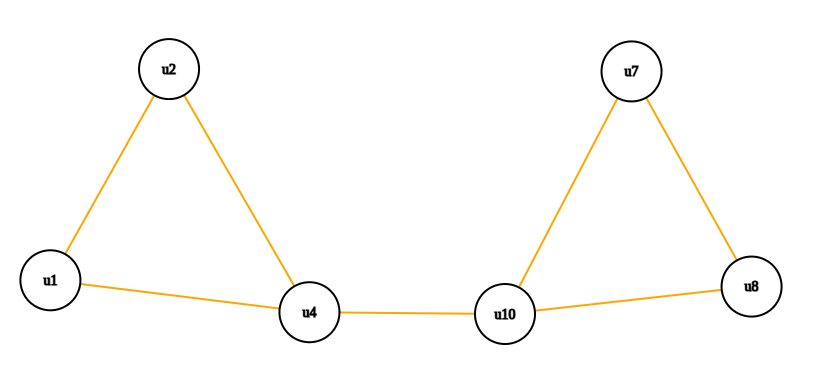
\includegraphics[width=1\textwidth]{assets/induced-subgraph.png}
              \caption{Subgráfica inducida por \( A \)}
              \label{fig:induced-subgraph}
          \end{figure}

    \item Di si las gráficas \( G_1 \) y \( G_2 \) son subgráficas inducidas de \( G' \). Argumenta tus respuestas.
          \begin{figure}[h]
              \centering
              \includegraphics[width=0.7\textwidth]{assets/g1.png}
              \caption{Gráfica \( G_1 \)}
              \label{fig:g1}
          \end{figure}
          \begin{figure}[h]
              \centering
              \includegraphics[width=0.7\textwidth]{assets/g2.png}
              \caption{Gráfica \( G_2 \)}
              \label{fig:g2}
          \end{figure}
          \textbf{Respuesta:} La gráfica \( G_1 \) es una subgráfica inducida de \( G' \), ya que las conexiones entre los vértices de \( G_1 \) son las mismas que las conexiones entre los vértices de \( G' \). Por otro lado, la gráfica \( G_2 \) no es una subgráfica inducida de \( G' \), ya que los vértices \( u_1 \) y \( u_2 \) están conectados en \( G_2 \), pero no en \( G' \).
\end{enumerate}


\section*{Problema 6}
Da un ejemplo de dos gráficas \( G \) y \( H \) y una función biyectiva \( f: V(G) \rightarrow V(H) \) tal que si \( uv \in E(G) \), entonces \( f(u)f(v) \in E(H) \), pero que \( G \) y \( H \) no sean isomorfas.

\end{document}
